\chapter{Methodology}

\section{General discussion on the decentralization of the controller}

In order to decentralize the controller, we need to recalculate the full force vector using only local observations

\begin{equation}
  f(t) = f_g(t) + f_\lambda(t)
  \label{eq:decentralized-force}
\end{equation}

$f_g$ is directly calculated from the load state and reference using a PID controller eq. \eqref{eq:error-position} to eq. \eqref{eq:desired-torque}, so no global observations about the other drone states are required.

$f_\lambda$ is a little bit more complicated, because it relies on a combination of the load state, drone velocities, and the optimizer’s internal state of $A$ and $\xi$, a phase shift assigned to each drone and time. The load state is locally observable to each drone so it is not an issue. The drone velocities are needed due to the nature of calculating $f_\lambda$. Since $f_\lambda(t) = N(H,t) \cdot \lambda(t)$ (eq.~\eqref{eq:il-nullspace-force}), the whole lambda vector is needed even just to calculate the $f_{\lambda_i}$ slice of one drone. This depends on the structure of matrix $N$ but for the purposes of this thesis it is enough to say that it is not diagonal. Therefore $f_{\lambda_i}$ is not only dependent on $\lambda_i$ but also on other $\lambda_i$'s. The lambda vector comes directly from the optimizer, the optimizer depends on the drone velocities and its own memory of the $A$, $\xi$ and the phase shift of each drone. The phase shifts are constant for a given configuration so the policy can just memorize it for each lambda. $A$ and $\xi$ are more intricate because they depend on the drone velocities. Precisely, any drop in the velocity of any drone leads to the increase of $A$ and $\xi$ for the whole formation. Making a neural network learn the internal states ($A$ and $\xi$) is possible either using smart design of the observation space if a Multi-Layer Perceptron (MLP) is used or using a Gated Recurrent Unit (GRU). In this work an MLP is chosen for phase one due to its simplicity and lightweight nature. To compensate for the lack of an internal state, multiple historical data points of specific features are stacked and fed together as input to the MLP, more on this will be discussed later. An approximation of the drones’ velocities can be analytically computed in a manner similar to what is done in [4]. This calculation uses as input: the observed load state, the commanded full force vector and its derivative, the commanded wrench and $\lambda(t)$ and its derivative. The resulting velocities will remain reasonably accurate as long as the drones agree on the load state measurement. For phase one, this agreement is assumed. These calculated velocities can then be fed into the MLP as a proxy for global information.

Lastly, while the optimizer uses time explicitly, it is not actually needed, what is actually needed is to time the periodic nature of the lambdas. This policy can learn this periodicity again using intelligent observation space design, by feeding multiple historical data points of specific features and by using time embedding techniques such as Fourier time encoding, this idea will be discussed in detail in a later section.  

By employing all these techniques together, we can reasonably aim to train an MLP using Behavioral Cloning (BC) to learn mimicking the optimizer. This MLP can then be deployed on each drone separately. It will output the full lambda vector, and then we calculate the full force vector using the classical pipeline math. Finally, each drone applies its own slice of the force vector, this requires that each drone knows its ID in order to know which slice to select. But this information can be communicated/agreed upon only once in the beginning.

This achieves two major advantages over the optimizer:

\begin{itemize}
  \item We cut the runtime dramatically. Optimizer takes \textasciitilde{}3-4 ms/step (benchmarked on an Intel(R) Core(TM) i7-10750H CPU @ 2.60GHz with 16GB of RAM) while a trained NN inference time takes $\ll$ 1ms/step on any modern GPU.\footnote{The theoretical compute time, based on FLOP count and peak GPU throughput, is on the order of microseconds. However, in practice, the total inference latency would be dominated by GPU overhead}
  \item Cutting the runtime is not only necessary for onboard deployment but also practically a requirement if we want to do Residual RL on top of the whole pipeline as in phase 2. In order to do RL we need to simulate millions of steps, therefore any extra computational cost per step quickly adds up. A single component in the pipeline taking 3-4 ms makes the RL practically infeasible.
\end{itemize}

\begin{itemize}
  \item We can do RL and warm start our actor from this behaviorally cloned policy so we can mold it to our needs (if it turns out to be helpful or required). This was not pursued in the present work, but it could be considered in future work.
\end{itemize}

\section{Implementation details}

The system model/plant was developed entirely inside Simulink. It was then exported as an FMU that python can step through to develop the optimizer on top (using CasADi). The FMU can also be wrapped in a gymnasium environment to allow easy interface with PyTorch for IL and RL. However, the FMU cannot be run on GPU directly so the number of parallel environments is limited by the CPU cores. This was chosen because the modeling of cable-suspended multibody systems is susceptible to subtle formulation and implementation errors when performed manually. In contrast, Simulink provides a framework that facilitates the consistent and accurate formulation of such systems. Since the PID controller, the optimizer were going to be developed on top of it. A reliable ground-truth plant to validate them necessary. Additionally, the main bottleneck in phase one was running the CasADi optimizer that the net needs to imitate. The optimizer runs on the CPU and takes 3-4ms/step while the FMU alone takes >1 ms/step. This means that parallelizing the environment and running thousands of instances on the GPU would be useless anyway. For phase 2 (the MARL phase), since the optimizer is not used anymore, the bottleneck shifted to simulating the environment. This marked the point at which the Simulink generated FMU choice became increasingly burdensome. However, it was still possible to train a prototype agent that demonstrates the feasibility of the proposed approach. For future work, the system model should be implemented within a GPU-parallelizable environment, such as JAX or NVIDIA Warp.

\section{Phase One : Imitation Learning}

\noindent\textbf{Initial approach}

As a starting point, we attempted a simple supervised learning setup. We generate a trajectory using the CCS (later referred to as the expert), we collect the inputs that we intend to feed the NN at each time step and finally we record the output $\lambda$ calculated by the expert. This creates a Dataset $\mathcal{D} = \{(s_i, a_i)\}_{i=1}^N$, where our state $s_i$ will be the input and action $a_i$ is the $\lambda$ output.

We can then train the policy neural network in a supervised learning setting, where regression is performed on expert state–action pairs.

As a first attempt, only one trajectory was used to simplify computational load and allows us to investigate whether the policy neural network (an MLP) can provide $\lambda$ and fly the carriers successfully in closed loop. The main challenge being that in this setting, the policy receives states generated by its actions as inputs during execution, rather than relying on expert-generated states. The trajectory was chosen with to ensure that the optimizer is engaged multiple times during the trajectory so that $\xi(t)$ and $A(t)$ meaningfully change. This is to ensure that the net captures a broad range of the optimizer’s behavior.

Figure 3: Components of the initial desired load trajectory used in the first attempt. The load starts from rest, follows a linear trajectory along the x-axis, and then comes to rest at its final position.

% (this belongs in Results, not Methodology, per earlier instruction -- left
% visible here for now rather than hidden, so it stays trackable in the PDF)

After the initial attempt proved successful and the policy was able to closely mimic the optimizer, the approach was generalized to a diverse set of trajectories, as will discussed in following sections.

\subsection{State/Input Design}

As discussed earlier, this is a critical design choice since the optimizer has many internal variables and the MLP has no memory element. Furthermore, $\lambda$ is not just a function of these internal states but also a function of time. Indeed, given fixed $\phi$, $\xi$ and $A$, $\lambda$ is still time varying since it is a sinusoid eq. \eqref{eq:lambda-def}. 

We can generally split the variables that $\lambda$ depends on to three main categories.

\begin{enumerate}
  \item Physical system states: these are either measured or estimated or a combination of both. For us, these are the carrier velocities.
  \item Internal variables: these are stored inside the optimizer and can either be fixed or be variable depending on the physical system states and their past value. For us, these are $\phi_i$, $\xi(t)$ and $A(t)$.
  \item Time: in order to build the sinusoid after determining all the internal variables. 
\end{enumerate}

We discuss each of them in turn in the remainder of this subsection.

\noindent\textbf{Physical system states}

Naturally, the reconstructed velocities of the carriers $\dot{p}_{R_i}$, $i = 1, \dots, n$ are a going to be part of the state. For our particular implementation we chose $n = 4$, so the first part of our state is $\dot{p}_{R_{1,2,3,4}} \in \mathbb{R}^{12}$ i.e. the carrier velocity vectors stacked. While technically only the velocity norms are needed, the whole vectors were provided thus increasing the information available to the MLP and allowing it to calculate the norm internally. 

\noindent\textbf{Internal variables}

The phase shifts $\phi_i$, $i = 1,2,3,4$ are constant for a given configuration and therefore can be memorized. On the other hand, $\xi(t)$ and $A(t)$ are variable and depend on their previous value and the carrier velocity norms. Since the initial value for them in the optimizer is constant, a reasonable assumption would be that the network can memorize them if they remain unchanged. But since they only change based on the carrier velocities (which are provided to the policy), the policy can just memorize the initial condition and learn to change them similar to the optimizer conditioned on the velocity norms. The challenge is MLPs don’t have any memory or internal state. Consequently, if the policy learns to change $\xi(t)$ and $A(t)$ in a given step based on its input and what the expert action was by the next step it will have no memory of this and will fall back to the default/initial $\xi(t)$ and $A(t)$ that structurally memorized. A reasonable remedy would be to supply the policy’s last action as part of the current state/input. So $a(t) \in s(t+1)$ or in our case $\lambda(t) \in s(t+1)$. 

For learning a single trajectory, this proved to be sufficient. However, during generalization it was not enough and the policy was not able to accurately mimic the optimizer. By analyzing its failure mode and the underlying causes, more history information was determined to be necessary (will be discussed in detail in the results section). As a result, instead of just supplying the last $\lambda$ as an input to the next time step, log-spaced point taps ($\lambda$ at lags 1, 2, 4, 8, 16, 32, 64, 128, 192, 256 steps) were used. 

This technique means we need to provide multiple historical $\lambda$'s that did not exist at $t=0$. To address this challenge, we assume that the initial $\xi(t)$ and $A(t)$ are agreed on once in the beginning (either by communication or just hardcoding) . They are then used to construct the historical $\lambda$'s by extrapolation in the past knowing the fixed phase shifts of the configuration. 

\noindent\textbf{Time}

Although providing the time directly to the NN may appear to be the most straightforward solution, this approach leads to several problems. First of all, during the initial stage when we are training on one trajectory, this risks that the network just memorizes which actions to do just based on time. This completely invalidates the test and compromises the investigation of whether the provided state is enough to make the actions learnable. Secondly, it creates generalization risks when we attempt to run episodes longer than those used in the training. Lastly, it creates normalization problems since we normalize our observation space before feeding it to the net, by using larger and larger time stamps we distort this normalization and destabilize the resulting observations. 

The main goal of using the time to determine the current phase in the sinusoid function. Consequently, we need only to encode the position in the oscillation. It can be argued that the previous $\lambda$ carries this information and therefore should be enough. However, this might be too demanding as any small perturbation or noise in the output can cause the NN to deviate and think it is in a different phase at the next time step. The perturbed output is used as input at the next time step, creating a feedback loop in which the resulting deviation can propagate and compound over subsequent steps. As the policy continues to act on increasingly perturbed observations, the instability can become self-reinforcing, while simultaneously driving the physical system away from its intended state. 

It is important to note that this information is not encoded in any way in the load position, as it can be completely static while $\lambda$ is oscillating. Nevertheless, an interesting observation is that since each carrier is always orbiting based on $\lambda$, its position and velocity implicitly encode its phase within the cycle. So the policy does not necessarily need to have access to time. The phase of the periodic signal is recoverable from the observable state of the system. In this sense, the dynamics of the environment effectively integrate the periodic signal into the carrier's physical state, allowing the policy to infer the corresponding phase of $\lambda$ directly from the observation rather than relying on an external clock. The main challenge with this approach, though, is that it suffers from the same sensitivity and instability as depending on $(t-1)$. Once the carrier position and velocity are perturbed or noised in any way, the policy’s inference of the phase can deviate in an unrecoverable way that is similar to what was described in the previous paragraph.

A promising solution would be to use the output of a periodic function in time. One possible function can be a saw tooth, but an even better solution can be using sine and cosine functions.  

\noindent\textbf{Fourier time encoding/ Fourier feature mapping}

Fourier time encoding (also called trigonometric clock embedding, sinusoidal time embedding, or Fourier feature encoding) is a way of representing time or phase as a vector of periodic functions instead of a single scalar [5].

\begin{equation}
  \phi(t) = [\sin(\omega t),\ \cos(\omega t)]
  \label{eq:fourier-basic}
\end{equation}

This anchors the observation in time, making any deviations recoverable. This observation is also immune to noise or perturbations. Sine and cosine are combined since sine alone (or cosine alone) cannot uniquely identify the phase.

$\sin(\theta) = \sin(\pi - \theta)$, so two different phases can produce the same value.

With both sine and cosine, each phase corresponds to a unique point on the circle/phase: $\theta \longrightarrow [\sin(\theta), \cos(\theta)]$.

Furthermore, instead of using just one frequency, we can use a set of frequencies $\{\omega_i\}_{i=1}^{K}$. 

\begin{equation}
  \phi(t) = [\sin(\omega_1 t), \cos(\omega_1 t), \sin(\omega_2 t), \cos(\omega_2 t), \dots, \sin(\omega_K t), \cos(\omega_K t)]
  \label{eq:fourier-general}
\end{equation}

This is because $\xi(t)$ can change from trajectory to another and within the same trajectory so the policy needs to learn to switch to a different frequency and time itself using it. Specifically, we use seven frequencies $\{1.5, 1.75, 2.0, 2.25, 2.5, 2.75, 3.0\}$ rad/s. These frequencies were selected based on observing $\xi(t)$ on a wide variation of trajectories. It was observed that $\xi(t)$ never dips below 1.5 rad/s and never goes above 3.0 rad/s, so that was the appropriate range to provide. A spacing of 0.25 rad/s was selected to create a densely spaced frequency set, providing a finer representation of temporal variations within our narrow frequency range while avoiding redundancy and excessive growth in the dimensionality of the input representation. This enables the network to better distinguish between closely spaced temporal frequencies without increasing the total number of frequencies unnecessarily.

\_\_\_\_\_Discuss risk of memorization\_\_\_\_\_\_\_

To summarize, the observation space can of the Imitation learning policy is:

\begin{itemize}
  \item Fourier time embedding/features (eq.~\eqref{eq:fourier-general} with $K=7$):
  \[
    \phi(t) = [\sin(\omega_1 t), \cos(\omega_1 t), \sin(\omega_2 t), \cos(\omega_2 t), \dots, \sin(\omega_7 t), \cos(\omega_7 t)]
  \]
  \item Reconstructed carrier velocities:
  \[
    \dot{p}_{R_i}(t), \quad i=1,2,3,4
  \]
  \item Log-spaced point taps ($\lambda$ at lags 1, 2, 4, 8, 16, 32, 64, 128, 192, 256 steps):
  \[
  \begin{gathered}
    [\lambda(t-1), \lambda(t-2), \lambda(t-4), \lambda(t-8), \lambda(t-16), \\
     \lambda(t-32), \lambda(t-64), \lambda(t-128), \lambda(t-192), \lambda(t-256)]
  \end{gathered}
  \]
\end{itemize}

\subsection{Dataset Aggregation (DAgger)}

While normal BC provides a simple and effective way to learn a policy from expert demonstrations by treating imitation learning as a supervised learning problem. The key assumption, however, is that the states encountered by the learner during deployment will look similar to those seen in the expert demonstrations.

In practice, this assumption often breaks down. A small mistake by the learned policy can take the agent into a state that the expert never visited. Since the policy has not learned how to act in these unfamiliar states, its errors can compound, causing it to drift further away from the expert's trajectory. This is known as covariate shift or the distribution mismatch problem [6].

DAgger addresses this issue by making the learner interact with the environment and querying the expert for the correct action on the states that the learner actually encounters. These newly labeled states are then aggregated with the original demonstrations to retrain the policy [6].

Thus, while BC learns to imitate the expert on the expert's state distribution, DAgger trains the policy on the states it is likely to encounter itself. This makes DAgger particularly useful for reducing compounding errors and improving robustness when the learned policy deviates from the expert.

Moreover, we do not suddenly expose the policy to its completely off-distribution states. We want to stay near the good orbit while slowly letting the policy explore off it. To accomplish that, DAgger defines the rollout/data-collection policy as

\begin{equation}
  \pi_i = \beta_i \pi^* + (1-\beta_i)\hat{\pi}_i,
  \label{eq:dagger-mixing}
\end{equation}

where:

\begin{itemize}
  \item $\pi^*$ = expert policy
  \item $\hat{\pi}_i$ = current learned policy
  \item $\beta_i$ = mixing parameter $\beta$
\end{itemize}

Unlike the original DAgger formulation, where the expert and learner policies are selected stochastically according to the mixing probability $\beta$, we use $\beta$ as an interpolation coefficient to directly combine their actions. Thus, the executed action is obtained as a weighted combination of the expert and learner actions. 

This continuous interpolation is well suited to a control setting that operates in a continuous action space. 

Additionally, at each DAgger iteration, $\beta$ is gradually decreased from 1 to 0 (e.g., in decrements of 0.1), resulting in a smooth transition from expert-guided behavior to the learned policy. For each value of $\beta$, data are collected using the resulting mixture of expert and learned actions and subsequently added to the aggregated dataset. The policy network is then retrained from scratch on the entire aggregated dataset before proceeding to the next iteration.

In this implementation, the $\beta$ schedule that was used is: $[0.9, 0.8, 0.7, 0.6, 0.5, 0.4, 0.3, 0.2, 0.15, 0.1, 0.08, 0.06, 0.04, 0.02, 0.0]$

The smaller $\beta$ closer to the end is to make the transition to policy closed loop control as smooth as possible.

The DAgger iteration can then be summarized in three steps: 

\begin{enumerate}
  \item Collect experience using
  \[
    \pi_i = \beta_i \pi^* + (1-\beta_i)\hat{\pi}_i \quad \text{(eq.~\ref{eq:dagger-mixing})}
  \]
  \item Aggregate the collected experience with the total dataset and train on it
  \item Decrease $\beta$ and repeat
\end{enumerate}

\begin{figure}[htb]
  \centering
  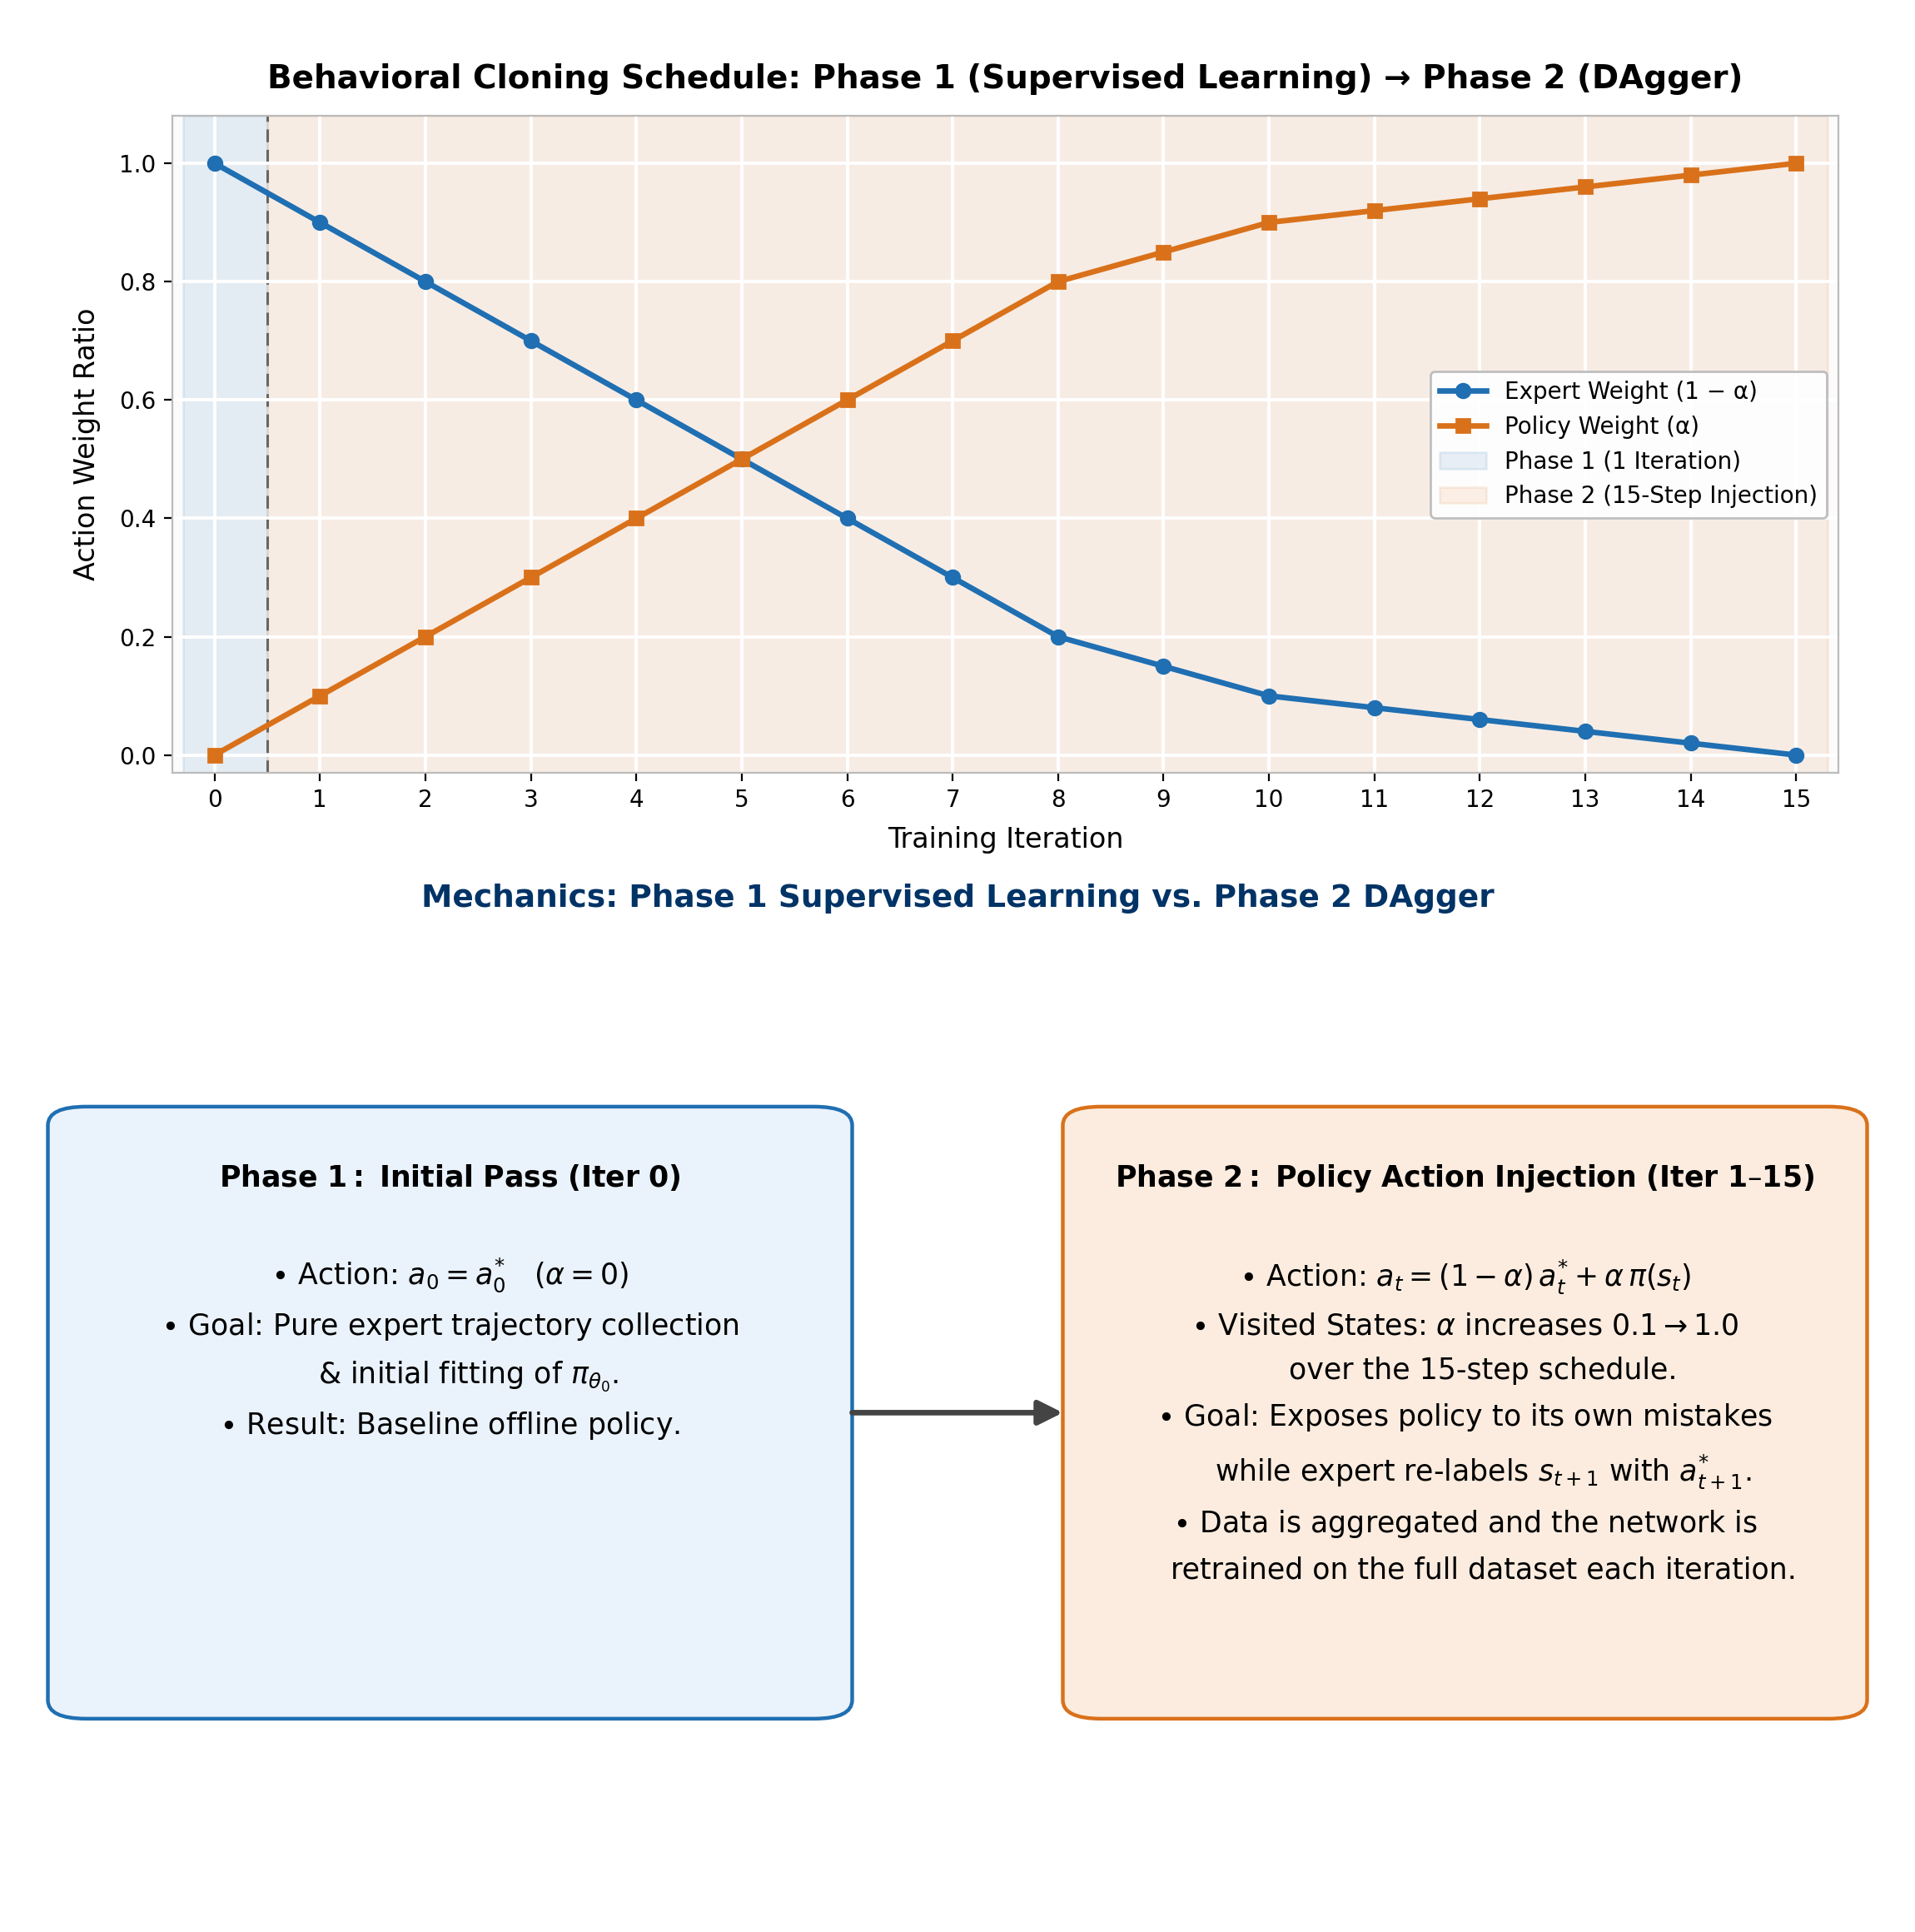
\includegraphics[width=\textwidth,height=14cm]{figures/fig-bc-dagger-schedule.png}
  \caption{Behavioral Cloning Schedule: Phase 1 (Supervised Learning) $\rightarrow$ Phase 2 (DAgger).}
  \label{fig:bc-dagger-schedule}
\end{figure}

Remark 2: The policy input $(\dot{p}_R, \lambda_{t-1})$ is reconstructed using the applied (mixed) $\lambda$ history, rather than the policy output alone. This is necessary because $\lambda_{t-1}$ represents a physical observation of the system state, specifically the cable force distribution that was actually applied to the system at the previous time step, rather than an internal memory state of the policy. Consequently, the observation at time $t$ must be consistent with the physical state generated by the applied action $\lambda_{\mathrm{applied},t-1}$. Using the policy output alone could instead produce a physically inconsistent state in which the kinematic variables reflect the response to one cable-force distribution, while $\lambda_{t-1}$ corresponds to another. Reconstructing the input from the applied $\lambda$ history therefore ensures that the policy is trained and evaluated on the state distribution it actually encounters during execution.

This strategy worked well when training on a single trajectory, however, during its extension to a much larger set of trajectories to achieve generalization, it became increasingly inefficient due to two main reasons: 

\begin{enumerate}
  \item Training the MLP from scratch each iteration
  \item Dataset size swelling
\end{enumerate}

The MLP is started from random weights at the beginning of each new DAgger iteration. This wastes many epochs to relearn stuff that can already exist in the old MLP weights. To counteract this, we warm-started each MLP from the previous DAgger iteration MLP.

However, this might increase the risk of being trapped in a local minima compounded by creating a sample imbalance in the dataset. To illustrate this, we consider the following numerical example.

Suppose each DAgger iteration rollout collects a dataset of size $N = 10000$

$\mathcal{D} = \{(s_i, a_i)\}_{i=1}^N$. By iteration 9, the old dataset $\mathcal{D}_{\text{old}}$ (has 90,000 samples) heavily outweighs the newly added rollout data $\Delta \mathcal{D}$ (10000 samples). The contribution of the newly added data to the learning becomes increasingly diminished especially towards the latter DAgger iterations. This is particularly harmful because the newly collected samples become increasingly representative of the state distribution encountered by the learned policy in the later iterations where $\beta$ approaches zero and the learner increasingly controls the system. Consequently, the policy may not sufficiently adapt to the newly encountered states, despite these being the most relevant for eventual deployment. While this might still happen even in the case of training the MLP from scratch, warm-starting from the last iteration MLP might further exacerbate this effect causing the MLP to become stuck in a local minimum. Utilizing the learning rate might not be suitable to mitigate this problem. By increasing it to escape the local minimum we risk destroying the features the MLP already learnt and then it becomes hard to fine tune. On the other hand, using a smaller learning rate means not being able to escape the local minimum. A dynamic learning rate can be used (higher in the beginning, decreases gradually), however, this was not needed since the upcoming point resolves the core issue.

The dataset size explodes towards the end, by the last couple of iterations the dataset size is more than 10x the original size. This problem became especially exacerbated during the generalization phase. The strategy is both inefficient because we need to train on too much data that is redundant and problematic due to the sample imbalance discussed earlier. A more efficient strategy is to train only on newly generated data or on a mix of new data and a representative sample of data from previous iterations.

The most valuable data for addressing covariate shift is collected in the final DAgger iterations, where $\beta \approx 0$ and the policy operates autonomously. These trajectories contain the states the learned policy actually visits, including realistic execution drift and recovery behaviors that are absent from the original expert demonstrations. As a result, they provide the strongest learning signal for the final policy.

In contrast, early iterations with $\beta = 0.9$ are dominated by expert intervention. The resulting samples are drawn primarily from $P(s \mid \pi_{\text{expert}})$ and are useful for initializing the policy, but they are less representative of the distribution encountered at deployment. Retaining all of this data throughout training therefore introduces substantial redundancy while contributing relatively little to the final behavior.

Reducing the dataset size offers two advantages: it lowers the computational cost of training and shifts the emphasis toward the distribution that matters most for autonomous control. A practical compromise is to retain all newly collected data from the final closed loop iterations while keeping only a representative subset of earlier data. For example, an 80\% new and 20\% sampled historical split preserves examples of recovery from rare, highly off nominal states without allowing redundant expert guided trajectories to dominate training.

The question then becomes how to choose the 20\% old data.

\textbf{Uniform:} Uniform random subsampling of the retained 20\% will, by chance, mostly keep easy data points, since that makes up most of any episode, and only occasionally keep the rarer, difficult maneuver data points. This is not ideal, especially towards the later iterations. As more iterations are added, the difficult examples from earlier iterations are increasingly diluted by the much larger number of easy, near-duplicate samples, making it less likely that uniform sampling will retain the data that is actually most informative for correcting the policy.

\textbf{Recency bias:} Sample more heavily from iterations that are more recent, since they are more representative of the policy's current behavior. However, depending on recency alone walks into the same trap of representing mostly easy data points. 

\textbf{Hardness bias:} If a data point is considered “easy,” e.g., the policy output and expert output are close, either dismiss it entirely or give it much less weight than “hard” points when sampling the old data. This proved to be less straightforward than it initially seemed, since the difficulty of a data point can be influenced by the history of deviations and errors that preceded it. In some cases, the state itself was not particularly difficult, but because it occurred after a sequence of errors, it appeared to be a hard example according to our criterion. This caused the MLP to learn overly aggressive corrective behaviors, which ultimately degraded performance even further (see the Results section for more details).

\textbf{Stratifying and binning:} Guarantee diversity by classifying points based on maneuver location, such as loitering, turning, moving in a straight line, etc. This can be done using reference velocity and acceleration, and then taking a certain percentage from each bin. The percentage could, for example, be determined by a hardness score for each bin.

Multiple test were conducted using these ideas and different combinations of them. The last two ideas, especially, were be mixed in different ways. For example, the data points within each bin would be selected or not based on difficulty to ensure good representation of both the different maneuvers and their difficulty levels. 

\noindent\textbf{Final Dataset Management Strategy}

Each DAgger iteration generates approximately \textbf{120K new data points}, which we label with \textbf{hardness, age, and bin/category}. We keep all of this new data for training and additionally augment it with uniformly sampled old data from a historical pool. When sampling the old data, we enforce a minimum representation per bin. If a bin would contribute less than the minimum 20\%, we sample additional points from that bin until this minimum is guaranteed.

The amount of old data sampled is around \textbf{65\% of the size of the new data}, resulting in a final training set of approximately \textbf{200K points}, with roughly \textbf{60\% new data and 40\% old data}. After training is completed, the new 120K points are added to the old data pool. Since the pool has a fixed size of \textbf{250K}, some data is then uniformly sampled for eviction to bring the pool back to its target size, again respecting the same minimum percentage per bin.

If the evaluation of a DAgger iteration proves to be unsatisfactory, based on metrics measuring how well the policy imitates the optimizer, the iteration is repeated with the same $\beta$. During this process, both the training dataset and the data pool are allowed to expand without any sampling, meaning that all available data is used for training and all data is kept in the pool. Once the policy reaches satisfactory performance, we shrink the datasets back to their normal sizes and resume the standard sampling procedure.

The bins are defined as:

\begin{itemize}
  \item \textbf{0 = Loiter:} reference speed $< V_{\mathrm{LO}} = 0.05\,\mathrm{m/s}$ (parked)
  \item \textbf{2 = Transition:} reference $|\mathrm{accel}| > A_{\mathrm{HI}} = 0.02\,\mathrm{m/s^2}$ (ramping)
  \item \textbf{1 = Cruise:} everything else (steady motion)
\end{itemize}

\begin{figure}[H]
  \centering
  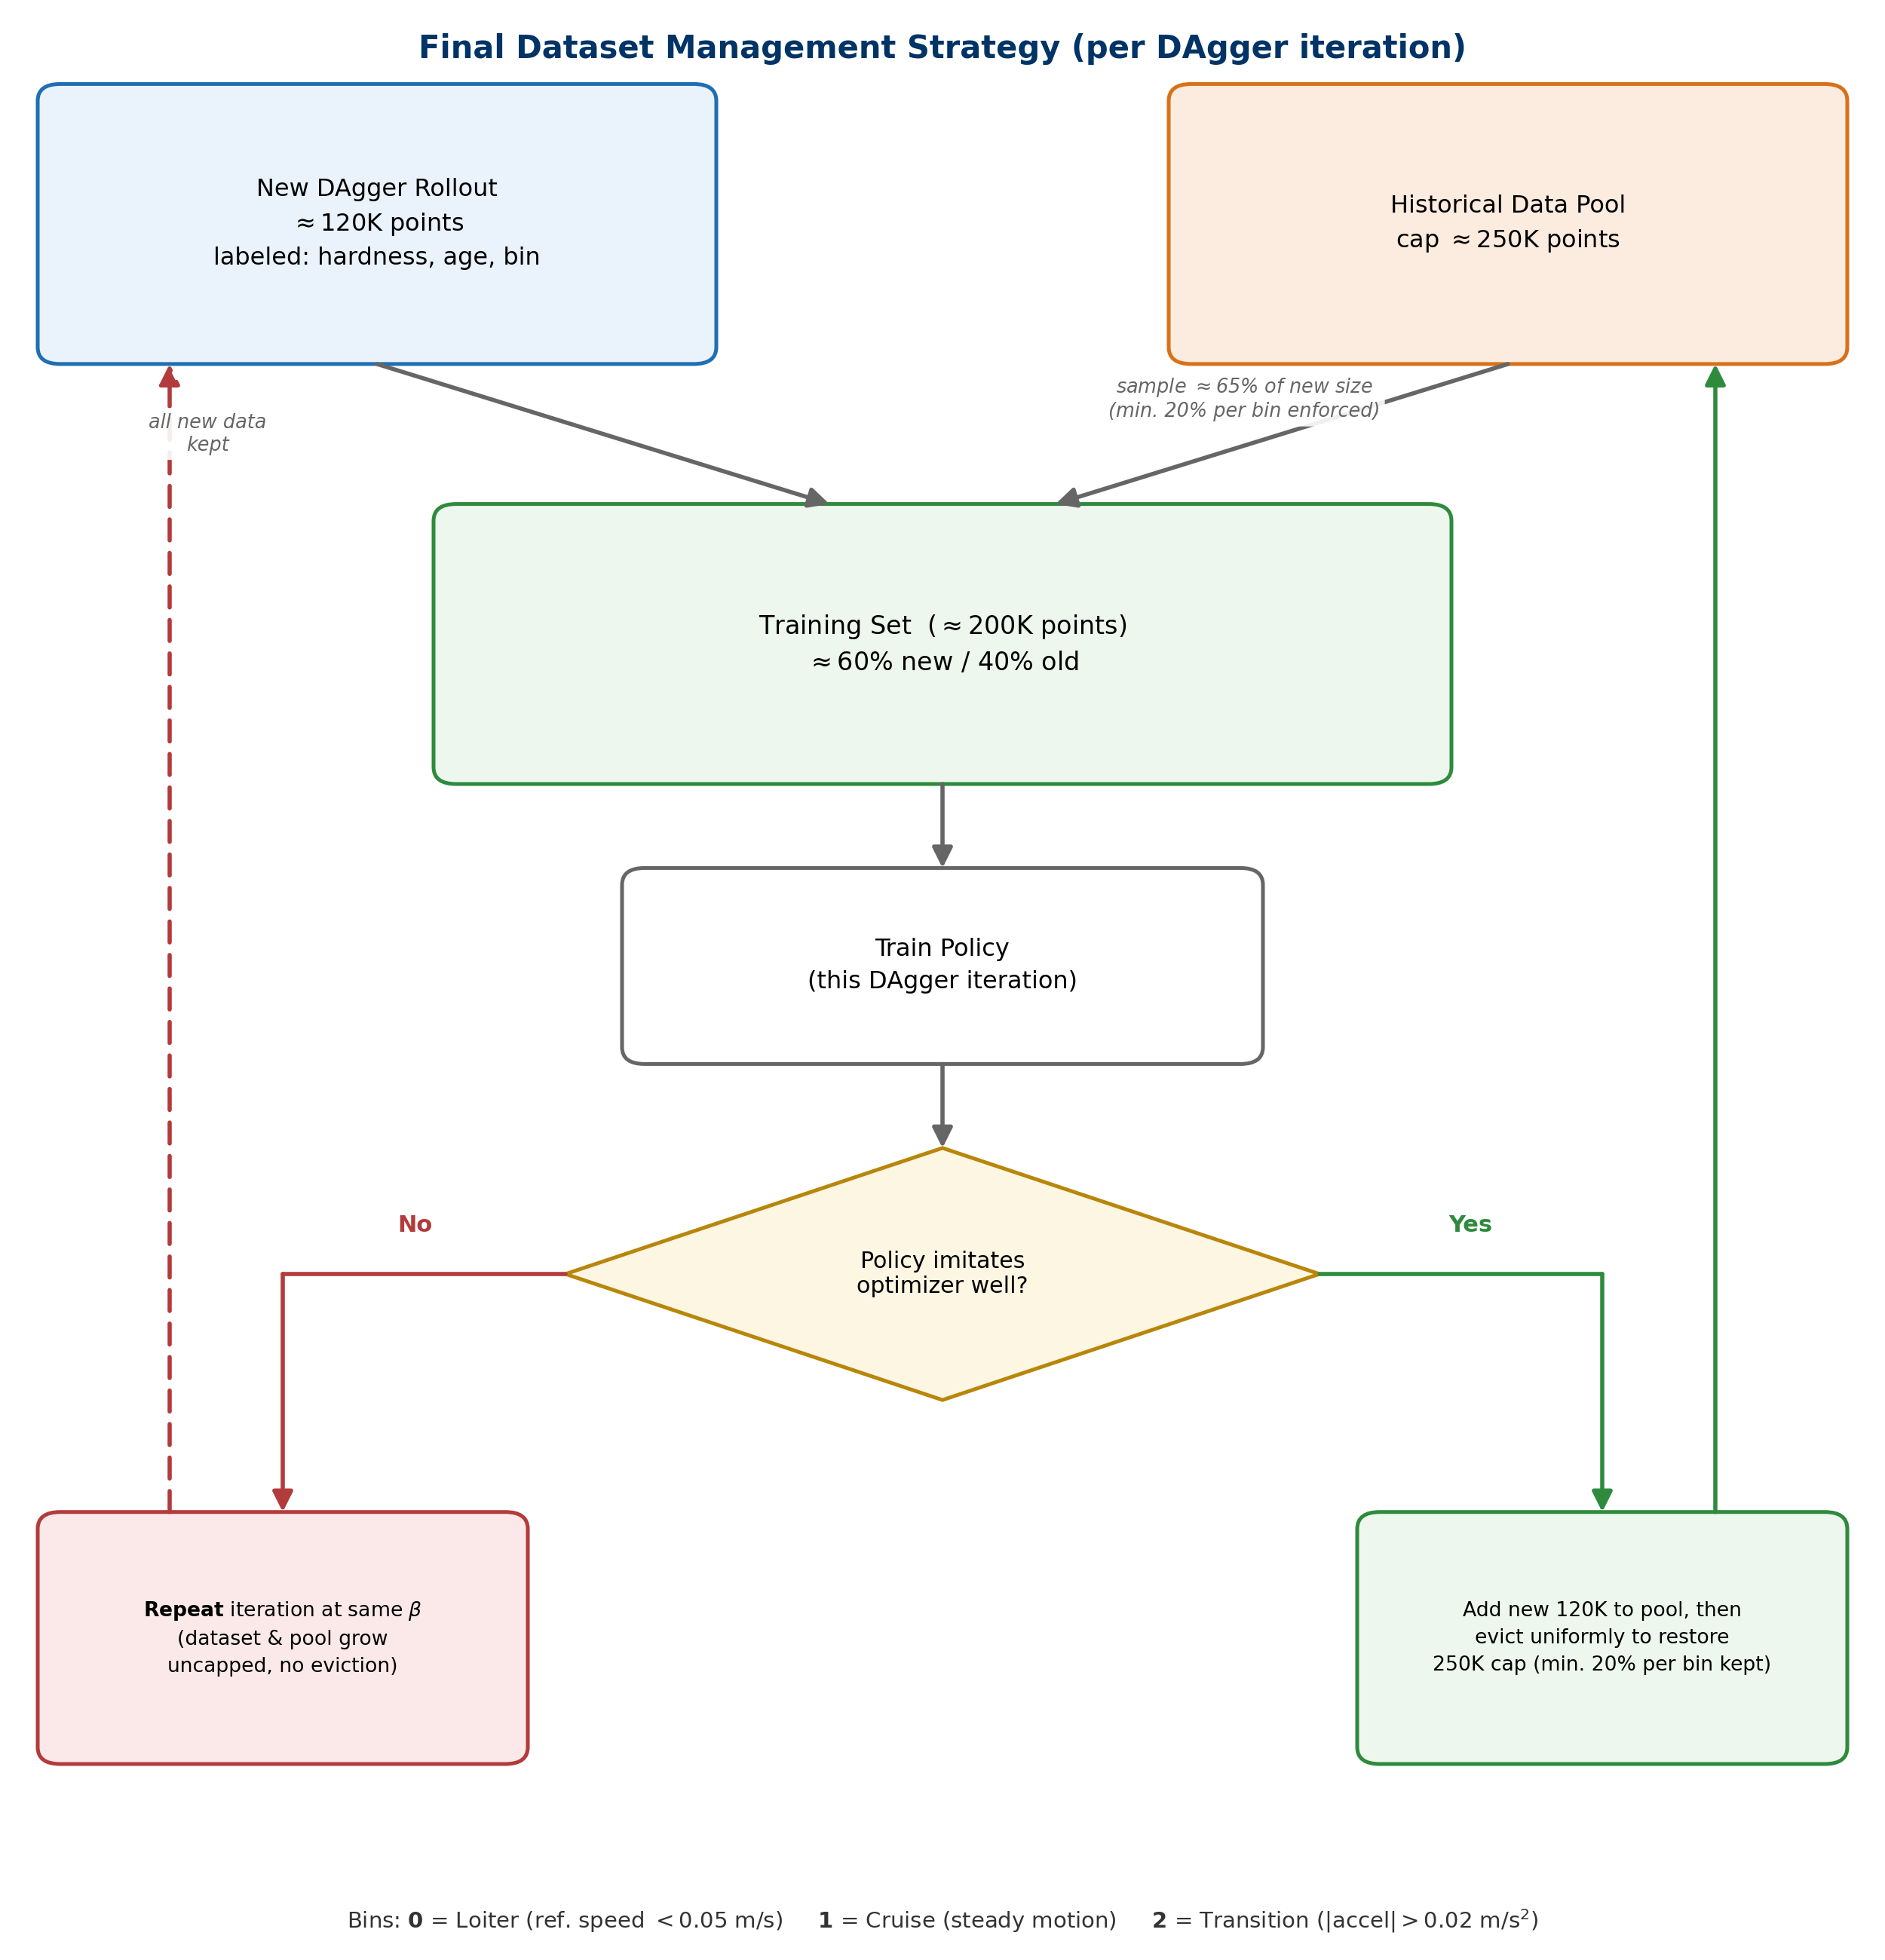
\includegraphics[width=\textwidth]{figures/fig-dataset-management.png}
  \caption{Final dataset management strategy per DAgger iteration: new rollout data and a bin-stratified sample of the historical pool form the training set; after a successful iteration the new data is merged into the pool and excess points are evicted uniformly (respecting the per-bin minimum) to restore the size cap.}
  \label{fig:dataset-management}
\end{figure}

\noindent\textbf{Evaluation metrics}

Two main metrics are used to determine whether a DAgger iteration was successful and we can safely move to a lower $\beta$ or not.

\noindent\textbf{Jitter}

For carrier i, we define jitter as

\begin{equation}
  J_i = \frac{1}{T-1} \sum_{t=1}^{T-1} \left| \lambda_i(t) - \lambda_i(t-1) \right|
  \label{eq:jitter-per-carrier}
\end{equation}

It is the mean absolute change between consecutive time steps of $\lambda_i$

\begin{itemize}
  \item $J_i = 0$ means the carrier outputs a perfectly constant coefficient throughout the episode.
  \item Larger $J_i$ means the policy changes its command more abruptly from one step to the next.
  \item There is no differentiation between increases and decreases from one step to the other since the absolute difference is used.
\end{itemize}

The team metric is simply the average across all drones:

\begin{equation}
  J = \frac{1}{N} \sum_{i=1}^{N} J_i
  \label{eq:jitter-team}
\end{equation}

Remark: this definition relies on our sampling period $\Delta t$ which is 10ms in our implementation.

Although we refer to this metric as jitter, it actually measures the mean absolute first difference of the action sequence. Consequently, it captures overall temporal variation in the policy output, including both abrupt fluctuations and smooth, gradual changes. Therefore, the optimizer’s smooth $\lambda$ has value $J \sim 0.016$ and we consider a policy to be smooth enough if its $J < 0.02$.

\noindent\textbf{Mean Squared Error}

For drone $i$, the mean squared error is:

\begin{equation}
  \mathrm{MSE}_i = \frac{1}{T} \sum_{t=0}^{T-1} \left( \lambda_i(t) - \lambda_i^{\mathrm{exp}}(t) \right)^2
  \label{eq:mse-per-carrier}
\end{equation}

Where $\lambda_i$ is the policy’s output and $\lambda_i^{\mathrm{exp}}$ is the optimizer’s output.

The team-level MSE is the average across all drones:

\begin{equation}
  \mathrm{MSE} = \frac{1}{N} \sum_{i=1}^{N} \mathrm{MSE}_i
  \label{eq:mse-team}
\end{equation}

An $\mathrm{MSE} < 10^{-3}$ is considered satisfactory.

\subsection{Generalization}

Once the policy was successful on one trajectory and the basic methodology proved to be functioning, the next step was to generalize by training on multiple trajectories. Training was done by sampling random component-wise rest-to-rest quintic polynomial trajectories. A validation/testing set was held out during training to evaluate the policy's ability to generalize to unseen trajectories. 

The generation of the random trajectories ensured generalization across movement scales, movement axes and episode durations. For example, testing was done on trajectories with displacements ranging from 0 to 20m along one or multiple axes. Furthermore, during training, episode durations were up to 35s, while the held-out test set included trajectories with durations of up to 75s. Thus, the evaluation included not only unseen combinations of movement magnitudes and axes, but also trajectories substantially longer than those encountered during training. This provides a test of whether the learned policy can maintain appropriate behavior over extended trajectories rather than relying on a fixed episode duration. Rotations were limited to the range of $[-10^\circ, 10^\circ]$ for each Euler angle to reduce the risk of system destabilization. 

\section{Phase Two : Reinforcement Learning}

\subsection{Introduction}

So far we have only discussed replicating the original centralized controller. We can, in theory, deploy it in a centralized manner assuming perfect knowledge of the system by all the carriers. Since they will agree on everything and they employ the same algorithm, coordination will be achieved implicitly without the need for communication. Each carrier will calculate the full force $f(t) = f_g(t) + f_\lambda(t) \in \mathbb{R}^{12}$ (eq.~\eqref{eq:decentralized-force}) and by knowing its ID, will apply its own slice from this vector $f_i(t) \in \mathbb{R}^3$. However, this property that might be helpful in theory to deploy the controller in a decentralized fashion instead makes deploying it under realistic assumptions quite delicate. The centralized controller uses global information on all the carriers to calculate $f(t)$. Specifically all the carrier velocities are needed to calculate $\lambda$. This global carrier information was reconstructed using load state and the total applied force $f(t)$. Once we have disagreements on the load state and the applied force (due to noise and delays/desynchronization), the reconstructed carrier velocities become completely corrupted and unreliable. This is on top of normal misalignments that will result from each carrier applying the controller to a different load state. While this is problematic, as long as the noise and desynchronization are bounded, the PID controllers will be able to stabilize the load. What is really insidious, is the disagreement in $\lambda$ due to the corruption of the global information. This estimation is not delicate and therefore the other carrier states become practically inaccessible. This is catastrophic as even a slight disagreement in $\lambda$ will continue to integrate over time and eventually lead to complete chaos and loss of coordination. To illustrate the issue, we consider the following example. 

Suppose carrier 1 receives a slightly noisy and delayed version of the load state. Based on that, it calculates a slightly inaccurate force. While this force might not significantly affect the load, it might cause its own velocity to drop below the aerodynamic threshold, $\varepsilon$. Based on that, its optimizer decides to increase $A$ and $\xi$. This is completely invisible to the other carriers, so their $A$ and $\xi$ remain constant. Over the next couple of seconds, a phase shift develops between the carriers’ internal forces, and they begin to no longer cancel each other out, causing the load to swing. As time goes on, the disagreement becomes catastrophic, and each carrier’s trajectory becomes completely uncoordinated with the others. This causes the carriers to crash into each other and the load to swing uncontrollably, as there is no feedback mechanism to make the carriers’ internal forces coordinate again.

Our goal is to deploy the same controller, while training a residual policy that corrects/augments its action. The objective would be to find a policy that can still maintain reasonable load tracking and coordinated carrier trajectories despite:

\begin{itemize}
  \item Noisy and asynchronous load state measurements
  \item Unreliable estimates of global information
\end{itemize}

Our setup is not simply attempting to use RL to produce better estimations of the global information; rather, it is investigating whether a learned policy can directly achieve robust decentralized behavior under the degraded information structure, without explicitly estimating or compensating for each agent's noisy and desynchronized observations.

In the results section, we argue that the policy achieves this goal by finding a control and coordination strategy that works under incomplete and noisy information, not by trying to “correct and denoise” this information.

\noindent\textbf{Overall Architecture}

Since we have multiple agents operating independently but all affecting the load together and affecting each other, the natural choice is to frame this problem as a Multi-Agent Reinforcement Learning (MARL) problem. Additionally, the performance of the carriers will be evaluated using a combination of global states (e.g. the true load position) and local states (e.g. carrier’s own velocity). Therefore, a Centralized Training with Decentralized Execution (CTDE) architecture was selected. This means that access to the global true centralized information is only available during the training evaluation process and not available to the individual carriers during the execution. We achieve this by using a shared/centralized critic with access to global state while the actor is deployed decentralized on each carrier. This means that during every time step, we have four actors taking actions in parallel. Since the carriers are identical and perform the same control task, differing only in their observations, we chose to share the same actor policy across them. This means that the four actors are homogeneous, using the same policy network and parameters, while producing actions based on their respective observations.

Furthermore, we use Multi-Agent Proximal Policy Optimization (MAPPO), akin to another work [7] that tackled a similar, yet distinct, decentralized multi-carrier cooperative payload transportation problem. While in [7] the carriers were multirotors that could hover, this work tackles non-stopping (fixed-wing) carriers. The MAPPO algorithm also aligns naturally with our chosen CTDE architecture. 

\subsection{Action Space}

Originally, the ideas was to keep wrench controller and optimizer and just add a residual $\delta f$ force to correct their behavior.

\begin{equation}
  f(t) = f_g(t) + f_\lambda(t) + \underline{\delta f(t)}
  \label{eq:phase2-naive-action}
\end{equation}

However, this means that the policy will be forced to learn the underlying force decomposition if it wants to act specifically in the internal forces for example. Instead of having the policy search until it discovers this division, it is more fruitful to make the action space work directly on both the wrench $w(t)$ and on lambda $\lambda(t)$.

\begin{equation}
  f(t) = G(t)^\dagger \cdot (w_d(t) + \underline{\delta w(t)}) + N(t) \cdot (\lambda(t) + \underline{\delta\lambda(t)})
  \label{eq:phase2-action-force}
\end{equation}

where $\delta w \in \mathbb{R}^6$ and $\delta \lambda \in \mathbb{R}^4$, total action space $\in \mathbb{R}^{10}$

This makes the policy gain insight into the underlying mechanics of the problem without having to discover it from scratch, as gradients on both $\delta w$ and $\delta \lambda$ are separate therefore learning how each one of them affects the system is 

\subsection{Observation Space}

The actor observation space must be limited to only local information (i.e. data that can be measured locally by sensors onboard the carrier). Additionally, in this work we assume no mid-flight communication, so the agent cannot have information about other carriers (unless they are mathematically reconstructed from local observations). 

\newpage
\noindent\textbf{Observation Space (Original\footnote{The use of the term “original” is clarified later in this section.}) $\in \mathbb{R}^{44}$}

\begin{itemize}
  \item Measured load state $\in \mathbb{R}^{18}$:
  \[
    [p_L(t), R_L(t), \dot{p}_L(t), \omega_L(t)]
  \]
\end{itemize}

Naturally the most important observation is the load state.

 Since there is no direct communication between the carriers, the load state is the only implicit way of information sharing between them. The underlying assumption is that the policy learns to use it to partially infer some information about the other carriers and consequently what its own action should be. 

\noindent\textbf{Noise and desynchronization}

To fully test the decentralization, we assume that every carrier makes its own measurement that is affected by its own noise and delay/desynchronization. 

The noise was modelled as an autoregressive Gaussian noise of order one $\mathrm{AR}(1)$. It represents temporally correlated estimation error. By tuning the correlation coefficient, it can represent a drifting, bias-like, viewpoint-dependent pose-estimation error. It was shown that this type of noise is more representative of realistic sensor noise rather than independent Gaussian white noise [8]. 

Additionally, each measurement is randomly delayed by $d_i \in [0, 2]$ time steps. Since our sampling period is 10 ms, this means that each measurement is delayed between 0 and 20 ms. $d_i$ is randomly chosen initially and evolves according to a random walk. This is done to represent asynchronous measurements by different carriers. The selected values are not derived from a specific empirical study; instead, they were chosen as reasonable estimates within the expected order of magnitude. A detailed characterization of these parameters is beyond the scope of this work since the characteristics of measurement delays and sensor noise can vary considerably depending on specific sensor and measurement setup [9].

\begin{itemize}
  \item Own carrier position and velocity $\in \mathbb{R}^6$:
  \[
    [p_R(t), \dot{p}_R(t)]
  \]
\end{itemize}

This observation is needed because we want to enable the policy to learn the orbiting behavior. Therefore, knowing the current position and velocity vector is necessary to determine the next action to maintain the orbiting behavior.  

\begin{itemize}
  \item Base force components $\in \mathbb{R}^6$:
  \[
    [f_g(t), f_\lambda(t)]
  \]
\end{itemize}

These are the forces the policy is supposed to augment/correct. Because the the policy is a residual one, it needs to know what the base controller is outputting in order to decide its appropriate action. The reason the force components are split is to provide specific information on what the base controller is doing both to the payload forces and to the internal forces. This also mirrors the action space structure.

\begin{itemize}
  \item Fourier time embedding/features $\in \mathbb{R}^{14}$:
  \[
    \phi(t) = [\sin(\omega_1 t), \cos(\omega_1 t), \sin(\omega_2 t), \cos(\omega_2 t), \dots, \sin(\omega_7 t), \cos(\omega_7 t)]
  \]
\end{itemize}

Similar to the observation space of the IL policy, the Fourier time embedding is   provided to the policy to anchor it in time, allowing it to learn the periodicity of the orbiting behavior without being able to explicitly memorize specific actions at specific times. Similar to the IL policy, we use seven frequencies $\{1.5, 1.75, 2.0, 2.25, 2.5, 2.75, 3.0\}$ rad/s based on the same reasoning. 

To summarize, the original observation space $\in \mathbb{R}^{44}$ and consists of:

\begin{itemize}
  \item Measured load state $\in \mathbb{R}^{18}$
  \[
    [p_L(t), R_L(t), \dot{p}_L(t), \omega_L(t)]
  \]
  \item Own carrier position and velocity $\in \mathbb{R}^6$
  \[
    [p_{R_i}(t), \dot{p}_{R_i}(t)]
  \]
  \item Base force components $\in \mathbb{R}^6$
  \[
    [f_g(t), f_\lambda(t)]
  \]
  \item Fourier time embedding/features
  \[
    \phi(t) = [\sin(\omega_1 t), \cos(\omega_1 t), \sin(\omega_2 t), \cos(\omega_2 t), \dots, \sin(\omega_K t), \cos(\omega_K t)]
  \]
\end{itemize}

Over the duration of this work, multiple experiments with different observation spaces were conducted. The goal of these experiments was not only to assess whether better performance can be achieved with different observation spaces, but also to shed some light on how the policy might be functioning.

For example, historical measurements were added for the load state and the carrier’s own position and velocity. However, this did not lead to an improvement in performance. The lack of benefit from additional historical information hints that the policy is not trying to estimate “more correct” global information. Instead, this suggests that the policy is finding control actions that work despite loss of information. Nevertheless, we include the augmented observation space as it was used to conduct many other experiments in the latter part of the work, on the possibility that it might lead to some minor improvement.

\noindent\textbf{Observation Space (Augmented) $\in \mathbb{R}^{98}$}

\begin{itemize}
  \item Original Observation Space in addition to:
  \item The last two measured load states $\in \mathbb{R}^{24}$
  \[
    [p_L(t-1), R_L(t-1), \dot{p}_L(t-1), \omega_L(t-1)]
  \]
  \[
    [p_L(t-2), R_L(t-2), \dot{p}_L(t-2), \omega_L(t-2)]
  \]
\end{itemize}

\begin{itemize}
  \item The last two own carrier position and velocity $\in \mathbb{R}^{12}$
  \[
    [p_R(t-1), \dot{p}_R(t-1)]
  \]
  \[
    [p_R(t-2), \dot{p}_R(t-2)]
  \]
\end{itemize}

\begin{itemize}
  \item Reference load state at current time $\in \mathbb{R}^{18}$
  \[
    [p_{Ld}(t), R_{Ld}(t), \dot{p}_{Ld}(t), \omega_{Ld}(t)]
  \]
\end{itemize}

As mentioned earlier, the goal of adding historical measurements of the load state and the carrier’s own position and velocity was to determine whether the policy can benefit from estimating better information about the system. Furthermore, the reference load state was added to give the policy insight about the base controller’s action and the possible direction of evolution of the load state in the next time step. We will show in the results section that these additions did not lead to any meaningful enhancement of the performance and we will comment further on what they mean.  

\noindent\textbf{Critic state $\in \mathbb{R}^{76}$}

Unlike the actor’s observation space, the critic’s state has access to global information that is true (not noisy or delayed). This allows it to objectively evaluate the actors’ actions and provide useful gradients for them to improve.

\begin{itemize}
  \item True load state $\in \mathbb{R}^{18}$:
  \[
    [p_L(t), R_L(t), \dot{p}_L(t), \omega_L(t)]
  \]
\end{itemize}

Used to assess whether the load is following its reference trajectory or not. 

\begin{itemize}
  \item All carriers’ positions $\in \mathbb{R}^{12}$:
  \[
    [p_{R_1}(t), p_{R_2}(t), p_{R_3}(t), p_{R_4}(t)]
  \]
\end{itemize}

\begin{itemize}
  \item All carriers’ velocities $\in \mathbb{R}^{12}$:
  \[
    [\dot{p}_{R_1}(t), \dot{p}_{R_2}(t), \dot{p}_{R_3}(t), \dot{p}_{R_4}(t)]
  \]
\end{itemize}

Carrier positions and velocities are used to determine if they are performing the orbiting behavior correctly or not. 

\begin{itemize}
  \item Expert-generated carriers’ positions $\in \mathbb{R}^{12}$:
  \[
    [p_{R_{e1}}(t), p_{R_{e2}}(t), p_{R_{e3}}(t), p_{R_{e4}}(t)]
  \]
\end{itemize}

Based on each carrier’s deviation from its respective expert trajectory, the critic should be able to evaluate how much degradation in the coordination between the carriers have occurred. The difference between the carriers’ actual state and expert calculated one generally the most affected/degraded metric when loss of coordination occurs and it is usually a good indicator on the overall health of the system. While the carriers are not required to follow the expert trajectory exactly, it is still useful as qualitative proxy for smooth orbiting. The expert generated trajectories are calculated based on a centralized controller + optimizer that get clean global information. For each training trajectory we calculate and store the expert trajectories for the carriers, they are then fed to the critic. The goal is to learn the underlying orbiting behavior in general, hoping that it will generalize this behavior to new trajectories. Since this information is only available to the critic during training, we do not need to worry about having to generate them at deployment. 

\begin{itemize}
  \item Delay of each carrier load measurement $\in \mathbb{R}^4$:
  \[
    [d_1, d_2, d_3, d_4]
  \]
\end{itemize}

Delays are added to critic state since they can make the state harder or easier, thus changing the expected reward, giving it to the critic helps making the advantage function more accurate. In other words, identical local observations by the carriers could correspond to different underlying difficulty based on how much desynchronization is between them. Therefore, to judge their actions and the resulting state of the system it is important for the critic to understand how delayed was each carrier, and how delayed they are with respect to each other.

\begin{itemize}
  \item Reference load state at current time $\in \mathbb{R}^{18}$
  \[
    [p_{Ld}(t), R_{Ld}(t), \dot{p}_{Ld}(t), \omega_{Ld}(t)]
  \]
\end{itemize}

Initially the reference load state was not provided to the critic. The rationale was that it will be able to infer it from the expert-generated carriers’ positions. While this proved to be true in our setup, it is not in general true, as the load has extra degrees of freedom based on the cables’ directions. However, in our setup with clean states the expert is able to drive the load with practically zero swinging, making the reference load state geometrically locked to the carriers’ state. In practice, the critic was able to learn this relationship quite well, as it was able to achieve excellent levels of accuracy (very low loss value), confirming our reasoning. Nevertheless, as a matter of principle, we still added it in the latter part of the work as a precaution, since the assumption might be violated at some point.

To summarize, the critic state $\in \mathbb{R}^{76}$ is composed of:

\begin{itemize}
  \item True load state $\in \mathbb{R}^{18}$:
  \[
    [p_L(t), R_L(t), \dot{p}_L(t), \omega_L(t)]
  \]
  \item All carriers’ positions $\in \mathbb{R}^{12}$:
  \[
    [p_{R_1}(t), p_{R_2}(t), p_{R_3}(t), p_{R_4}(t)]
  \]
  \item All carriers’ velocities $\in \mathbb{R}^{12}$:
  \[
    [\dot{p}_{R_1}(t), \dot{p}_{R_2}(t), \dot{p}_{R_3}(t), \dot{p}_{R_4}(t)]
  \]
  \item Expert-generated carriers’ positions $\in \mathbb{R}^{12}$:
  \[
    [p_{R_{e1}}(t), p_{R_{e2}}(t), p_{R_{e3}}(t), p_{R_{e4}}(t)]
  \]
  \item Delay of each carrier load measurement $\in \mathbb{R}^4$:
  \[
    [d_1, d_2, d_3, d_4]
  \]
  \item Reference load state at current time $\in \mathbb{R}^{18}$
  \[
    [p_{Ld}(t), R_{Ld}(t), \dot{p}_{Ld}(t), \omega_{Ld}(t)]
  \]
\end{itemize}

\subsection{Reward function}

The design of an efficient reward function is generally one of the most intricate challenges in RL. Fortunately, in the case of residual RL the challenge is slightly simplified since we already have a starting point. In this work, the design methodology was to observe failure modes of the existing setup and add terms one by one to steer the behavior away from these failure modes and towards desirable behavior. 

The per drone reward function is:

% NOTE: the formula below and several of the term definitions that follow were
% authored in this paragraph as native Word equation objects, which contain no
% plain text at all -- the original text-extraction pass (which only reads
% plain paragraph text) silently produced an empty paragraph for each one, so
% this content was completely missing until reconstructed from the document's
% underlying OOXML math markup.
\begin{equation}
  r_i = -\left( w_{\text{manifold}} d_i^2 + w_{\text{stall}} \,\text{stall}_i + w_{\text{load}} \|e_L\|^2 + w_{\text{overspeed}} \,\text{overspeed}_i^2 + w_{\text{overshoot}} \,\text{overshoot}_i \right)
  \label{eq:per-drone-reward}
\end{equation}

where $w_{\text{manifold}}$, $w_{\text{stall}}$, $w_{\text{load}}$, $w_{\text{overspeed}}$ and $w_{\text{overshoot}}$ are all strictly positive weights

And the team reward simply is:

\begin{equation}
  R_{\text{team}} = \sum_{i=1}^{N} r_i
  \label{eq:team-reward}
\end{equation}

Additionally, a penalty of $-100$ is applied once if any carrier’s speed exceeds $v_{\text{blowup}} = 100$. This also leads to the truncation of the episode 

In this subsection we break down each term one by one: 

\begin{itemize}
  \item \textbf{manifold ($d_i^2$):}
\end{itemize}

\begin{equation}
  d_i^2 = \|p_{\text{expert},i}(t) - p_i(t)\|^2
  \label{eq:manifold-term}
\end{equation}

Where $p_{\text{expert},i}(t)$ is the expert-generated trajectory for carrier $i$ at time $t$ (centralized controller with true states) and $p_i(t)$ is the actual carrier position. Naturally, this is a per carrier term. 

If there is no noise or desynchronization between the drones the value of this term should be zero. This term was added as a result of experimentation, so it is not required for the policy to follow the expert-generated trajectory exactly. However, it was discovered that it provides a useful feedback on the general health of the system. Usually it is low if the carriers are orbiting correctly and it is high if they are flying around uncontrollably or potentially crashing into each other. The squared absolute difference is used for this purpose, as it does not punish small magnitude deviations (minimizes their influence) while placing greater emphasis on bigger deviations.

\begin{itemize}
  \item \textbf{Aerodynamic stall ($\text{stall}_i$):}
\end{itemize}

\begin{equation}
  \text{stall}_i = d^2 + w_{\text{lin\_stall}} \cdot d
  \label{eq:stall-term}
\end{equation}

where $d = \max(0, (\varepsilon + \text{margin}) - \|v_i\|)$. $\varepsilon$ is the minimum flight speed before stall, margin is a small positive number to disincentivize approaching $\varepsilon$, $\|v_i\|$ is the velocity norm of carrier $i$, and $w_{\text{lin\_stall}}$ is a strictly positive weight

Again, this is a per carrier term. This term is a central reward term: no matter what the carriers do, they should never go below the aerodynamic stall speed $\varepsilon$. Therefore, this term was included from the outset and was not introduced as a result of experimentation. While some other terms are included to help shape the gradient and guide the policy toward good solutions, they are not inherently part of the requirements. This term, however, is a non-negotiable requirement. Therefore, this is reflected in the selection of its weights, which are chosen to be relatively high. Additionally, a margin was added to provide a buffer before reaching the actual stall velocity. Furthermore, linear and quadratic difference terms are used together to penalize violations immediately, even when they are small, while also greatly penalizing larger violations. The linear term is particularly important for small violations, for which the quadratic term alone would not provide a sufficiently strong penalty, while the quadratic term places greater emphasis on deep stalls. 

\begin{itemize}
  \item \textbf{load tracking error ($\|e_L\|^2$):}
\end{itemize}

Similar to the aerodynamic stall term, this term was included from the beginning as it is a main requirement of the system. Nevertheless, unlike the aerodynamic stall term, there is some leeway if the magnitude of the error is small. Accordingly, only quadratic error is used and no linear penalty is applied. This means that small magnitude errors are minimized while larger ones are emphasized. Moreover, this term is the only term that is shared between all the carriers. 

\begin{itemize}
  \item \textbf{Carrier Overspeed ($\text{overspeed}_i^2$):}
\end{itemize}

\begin{equation}
  \text{overspeed}_i^2 = \min\left(\text{over}^2 + w_{\text{overspeed\_linear}} \cdot \text{over}, \ \text{cap}_{\text{overspeed}}\right)
  \label{eq:overspeed-term}
\end{equation}

where $w_{\text{overspeed\_linear}}$ is a positive weight, $\text{over} = \max(0.0, \|v_i\| - \text{overspeed}_v)$, $\|v_i\|$ is the velocity norm of carrier $i$, and $\text{overspeed}_v$ is the upper bound of acceptable velocity norms and $\text{cap}_{\text{overspeed}}$ is an upper bound on the whole term value 

This term was added by observing how the base controller fails on many trajectories. In general, it was observed that a lack of coordination between the carriers can cause their speeds to increase dramatically, ultimately resulting in system blow-up, with speeds reaching unrealistic values (hundreds of m/s or more). We used the same combination of linear and quadratic penalties as before to discourage both small and big violations. Additionally, this term was capped to an upper value to prevent the advantage values, returns and ultimately the PPO update from becoming numerically unstable. This is because, as mentioned earlier, the carriers’ velocities can sometimes spike to arbitrary large values. This penalty is applied per carrier to only penalize the carrier that is accelerating. 

\begin{itemize}
  \item \textbf{$\delta\lambda$ cap overshoot ($\text{overshoot}_i$):}
\end{itemize}

\begin{equation}
  \text{overshoot}_i = \min\left(\text{over}_{\lambda,i}^2 + \text{over}_{\lambda,i}, \ \text{cap}_{\text{overshoot}}\right)
  \label{eq:overshoot-term}
\end{equation}

where $\text{cap}_{\text{overshoot}}$ is an upper bound on the whole term value, $\text{over}_{\lambda,i} = \max(0, \text{sat}_{\lambda,i} - 1)$, $\text{sat}_{\lambda,i} = \|\delta\lambda_i\|_2 / (\kappa_\lambda \cdot \|\lambda_{i,\text{base}}\|_2)$, and $\kappa_\lambda$ the allowable fraction of the base controller magnitude

In order to prevent the residual policy from taking arbitrarily large actions, $\delta\lambda$ and $\delta w$ were capped to a fraction $\kappa_\lambda$ of the base controller values. This prevents the policy from driving the system to instability while still allowing it to explore all the possible action space without being penalized for it.  However, during the training procedure, as the policy gets exposed to less-explored trajectories, it can start by outputting actions that are higher than these bounds. This causes a problem of dead gradients; decreasing or increasing the action slightly doesn’t lead to any change in the system’s behavior so the policy is not able to learn. Consequently, the goal of this penalty is to discourage the policy from outputting values that exceed the bound, even if such values were reached inadvertently. This problem was only observed for $\delta\lambda$ so the penalty is only applied there. $\delta w$ always stayed below its upper bound. 

The following is a table summarizing each term: 

\begin{longtable}{|p{0.22\textwidth}|p{0.38\textwidth}|p{0.30\textwidth}|}
\hline
\textbf{Term} & \textbf{Expression} & \textbf{Role} \\ \hline
\textbf{manifold ($d_i^2$)} & $\|p_{\text{expert},i}(t) - p_i(t)\|^2$ & Stay on the expert loiter loop (generated from ground truth states). The goal is not to follow it exactly, but to learn the underlying orbiting behavior in general. \\ \hline
\textbf{$\text{stall}_i$} & Graced hinge below cruise floor: \par $d^2 + w_{\text{lin\_stall}} \cdot d$, where $d = \max(0, (\varepsilon + \text{margin}) - \|v_i\|)$ & Fixed-wing stall floor (prevents airspeed drop) \\ \hline
\textbf{load tracking error} & $\|e_L\|^2$ & Keep the load on reference \\ \hline
\textbf{$\text{overspeed}_i^2$} & $\min(\text{over}^2 + 2 \cdot \text{over}, 75)$ \par where $\text{over} = \max(0.0, \|v_i\| - \text{overspeed}_v)$ & Prevent carrier from speeding up unnecessarily. Blowup guardrail. \\ \hline
\textbf{$\text{overshoot}_i$} & $\min(\text{over}_{\lambda,i}^2 + \text{over}_{\lambda,i}, 9)$ \par where $\text{over}_{\lambda,i} = \max(0, \text{sat}_{\lambda,i} - 1)$ \par and $\text{sat}_{\lambda,i} = \|\delta\lambda_i\|_2 / (\kappa_\lambda \cdot \|\lambda_{i,\text{base}}\|_2)$ \par $\kappa_\lambda$: the allowable fraction of the base controller magnitude & Prevents the policy from taking actions above the allowed fraction of the base controller magnitude (dead gradient, no learning). The cap prevents the policy from taking overly aggressive actions. \\ \hline
\end{longtable}

\textbf{Truncation Condition}: A one-shot penalty of $-100$ is triggered on a guard-truncated step if speed exceeds $v_{\text{blowup}} = 100$.

\subsection{Centralized Controller Policy Guidance experiment (using Supervised Learning)}

To test whether the policy is learning to recover the centralized controller behavior or genuinely learning a different decentralized reactive policy, we conducted an experiment in which we warm-started the policy network from a network that was trained using supervised learning to output $\delta\lambda^*$ and $\delta w^*$. Where $\delta\lambda^* = \lambda_{\text{base}} - \lambda_{\text{expert}}$. $\lambda_{\text{base}}$ is the controller output when it is deployed decentralized on noisy and asynchronous measurements, while $\lambda_{\text{expert}}$ is the centralized controller output using clean (no noise and in sync) states and global information. Furthermore, during training, the supervised learning loss term was added to the PPO loss terms. This provides a consistent gradient signal to the policy, encouraging it to learn solutions that recover the behavior of the centralized controller. However, as will be discussed in the results section, this approach was not effective and was therefore abandoned. 

\subsection{MAPPO implementation details}

In this section we go over some design choices that we consider noteworthy. We do not go over all the MAPPO algorithm details as this is not the main focus of this work.

\noindent\textbf{Advantage Estimates}

For each of the four agents, a separate advantage estimate is computed using its individual reward and the shared global value estimate:

\begin{equation}
  A_t^i = \operatorname{GAE}(r_t^i, V(s_t)).
  \label{eq:advantage-estimate}
\end{equation}

Thus, the critic provides a common assessment of the team's expected future performance from the complete global state, while the individual reward determines how the contribution of each agent is reflected in its corresponding advantage. This allows the four agents to share a common global assessment while retaining distinct learning signals based on their individual contributions.

\noindent\textbf{Critic Target}

The target used to train the critic is computed as the mean of the individual agent rewards, together with the value estimate of the subsequent state:

\begin{equation}
  y_t = \frac{1}{4}\sum_{i=1}^{4} r_t^i + V(s_{t+1}).
  \label{eq:critic-target}
\end{equation}

This provides the critic with a target that reflects the collective performance of the four agents while accounting for the expected future return.

\_\_\_\_Figure here from the ppt: Overview of MAPPO Training Loop and Environment Step\_\_\_

\noindent\textbf{Curriculum training}

Training the policy on the full set of trajectories simultaneously, with all reward terms active, proved challenging due to the diversity of behaviors and operating conditions. To facilitate policy learning, a curriculum training strategy was therefore adopted, in which both the training trajectories and reward terms were progressively expanded during training. This allows the policy to first learn from a more limited set of trajectories with simpler objectives before being exposed to increasingly diverse scenarios and more complex objectives.

Training on multiple trajectories together proved to be especially difficult, as the reward becomes extremely high variance, making the learning incredibly slow. This was not an issue of observation aliasing since the load reference trajectory is provided in the observation space. It is also not a network capacity since multiple attempts to increase the size of the MLP were made and the problem persisted. To combat this high variance, the policy was first trained on a single trajectory until mastery, and then more trajectories were added one by one. However, this still proved to be challenging and does not force the policy to learn to generalize. To ensure the correct diagnosis of the problem, and to explore a potential solution, we conducted the experiment illustrated in the next subsection.

\noindent\textbf{Behavior Cloning (BC) of multiple policies}

 In order to test whether the policy is unable to learn multiple trajectories together due to observation aliasing or network capacity, multiple teacher policies $\{\pi_1,\dots,\pi_K\}$ were first trained separately on different trajectories until mastery. After that, their combined input-output pairs were used to train a single student policy/network of the same architecture using BC. 

The combined dataset is: 

\begin{equation}
  \mathcal{D} = \bigcup_{i=1}^{K} \{(o_t, \pi_i(o_t))\}
  \label{eq:bc-combined-dataset}
\end{equation}

where $o_t$ is the observation and $\pi_i(o_t)$ is the teacher policy action

The single student policy $\pi_\theta$ with the same architecture and capacity is trained on $\mathcal{D}$ by minimizing the supervised imitation loss

\begin{equation}
  \mathcal{L}_{\mathrm{BC}}(\theta) = \mathbb{E}_{(o,a)\sim\mathcal{D}}\left[-\log \pi_\theta(a \mid o)\right].
  \label{eq:bc-loss}
\end{equation}

If the student policy is able to mimic the combined behavior of all teacher policies, this suggests that the main challenge is learning the policy, rather than the problem being inherently ill-posed or requiring a larger or more complex network. Additionally, since the combined student policy was trained using supervised learning in open loop, it might not be able to achieve the same performance as the teacher policies when deployed in closed loop. Instead of resorting to DAgger or other IL methods, the combined student policy can be used to warm-start a policy to be fine-tuned with RL to improve its behavior across the full set of trajectories mastered by the teacher policies. This process can later be iteratively repeated by combining the resulting policy with other policies that were trained in the same way, until generalization is achieved.

\_\_\_\_Figure here showing how RL policies are combined using IL then RL for fine tuning then a bigger IL combining combined policies and so on?\_\_\_\_\_

In results : It’s not learning to estimate (history doesn’t help + I attempted forcing it to learn the “correct” output using the loss) so it’s truly learning a decentralized reactive strategy.
